\documentclass[a4paper,12pt]{article}
%	options include 12pt or 11pt or 10pt
%	classes include article, report, book, letter

%% Always need these
\usepackage[utf8]{inputenc}
\usepackage[a4paper,pagebackref,hyperindex=true]{hyperref} % load hyperref before algorithm!!!!!!!
\usepackage{subfigure}
\usepackage{algorithm}
\usepackage{algorithmic}
\usepackage{amsmath}
\usepackage{fancyhdr}

%% Colored links in pdf
\usepackage{color}
\newcommand{\blue}{ \color{blue} }
\definecolor{linkcol}{rgb}{0,0,0.4}
\definecolor{citecol}{rgb}{0.5,0,0}

%% Bibliography text
% nicer backref links
\renewcommand*{\backref}[1]{}
\renewcommand*{\backrefalt}[4]{%
\ifcase #1 %
(Not cited.)%
\or
(Cited on page~#2.)%
\else
(Cited on pages~#2.)%
\fi}
\renewcommand*{\backrefsep}{, }
\renewcommand*{\backreftwosep}{ and~}
\renewcommand*{\backreflastsep}{ and~}

%% Language
\usepackage[ngerman,english]{babel}
\selectlanguage{ngerman}

%% Fonts
\usepackage[T1]{fontenc}
\usepackage{amsfonts} % need for mathbb
\usepackage[font=footnotesize,labelfont=bf]{caption} % small captions
%
% Latin Modern
%\usepackage{lmodern}
%
% Computer Concrete
%\usepackage{concmath}
%
% Utopia Regular with Math Design
%\usepackage[adobe-utopia]{mathdesign}
%
% Charter
\usepackage{charter}

%% Code
\usepackage{listings}
\lstset{ %
  language=C++, % choose the language of the code
  basicstyle=\small\ttfamily, % the size of the fonts that are used for the code
  numbers=left, % where to put the line-numbers
  numberstyle=\small\ttfamily\color[rgb]{0.6,0.6,0.6}, % the size of the fonts that are used for the line-numbers
  stepnumber=1, % the step between two line-numbers. If it's 1 each line
  xleftmargin=4mm,
  % will be numbered
  numbersep=5pt, % how far the line-numbers are from the code
  backgroundcolor=\color{white}, % choose the background color. You must add \usepackage{color}
  showspaces=false, % show spaces adding particular underscores
  showstringspaces=false, % underline spaces within strings
  showtabs=false, % show tabs within strings adding particular underscores
%  frame=l, % adds a frame around the code
  %frame=single,
  tabsize=2, % sets default tabsize to 2 spaces
  breaklines=true, % sets automatic line breaking
  breakatwhitespace=false, % sets if automatic breaks should only happen at whitespace
  % also try caption instead of title
  escapeinside={@}{@}, % if you want to add a comment within your code
  morekeywords={*,...}, % if you want to add more keywords to the set
  keywordstyle=\color[rgb]{0,0,1},
  commentstyle=\color[rgb]{0.133,0.545,0.133}\textit,
  stringstyle=\color[rgb]{0.627,0.126,0.941},
}

%% Customizations
\newenvironment{packed_item}{
\vspace{-2mm}
\begin{itemize}
  \setlength{\itemsep}{1.5pt}
  \setlength{\parskip}{0pt}
  \setlength{\parsep}{0pt}
}{\vspace{-2mm}\end{itemize}}

\newenvironment{abstr}{%
\vfill\small%
\begin{center}%
{\bfseries \abstractname}%
\end{center}%
\quotation}%
{\vfill}%

\newenvironment{todocontent}{%
\begin{outline}
\color[rgb]{0.6,0.6,0.6}
}{%
\end{outline}
}% End environment

% Provide the \*matter commands in non-book classes
\providecommand{\frontmatter}{%
\clearpage%
\pagenumbering{roman}%
\setcounter{page}{1}}%

\providecommand{\mainmatter}{%
\clearpage%
\pagenumbering{arabic}%
\setcounter{page}{1}%
\pagestyle{fancy}%
\fancyhf{}%
\fancyhead[L]{\leftmark}%
\fancyhead[R]{\thepage}%
}%

\providecommand{\backmatter}{%
\clearpage%
\pagenumbering{arabic}%
\setcounter{page}{1}}%

% Paragraph Intendation
\setlength{\parindent}{0pt}
\setlength{\parskip}{2ex}

%% todonotes. gives command \todo{do this thing}
\usepackage{todonotes}

%% Outlines
\usepackage{outlines}

%% Include macros
%% general vector style (bold or with arrow)
\newcommand{\ve}[1]{
    \mathbf{#1}
    %\vec{#1}
}

%% Specific to this thesis
\newcommand{\eps}{\varepsilon}

%% common shortcuts
\providecommand{\argmin}{\operatorname*{argmin}} % operatorname makes _{..} appear centered
\providecommand{\argmax}{\operatorname*{argmax}} % operatorname makes _{..} appear centered
\newcommand{\dd}[1]{\,\mathrm{d}#1} % integration: \int f(x) \dd{x}
\newcommand{\EE}{\mathbb{E}}        % expectation value
\newcommand{\RR}{\mathbb{R}}        % set of real numbers
\newcommand{\CC}{\mathbb{C}}        % set of complex numbers
\newcommand{\NN}{\mathbb{N}}        % set of natural numbers
\newcommand{\OO}{\mathcal{O}}       % big O notation (asymptotic complexity)
\newcommand{\TT}{\mathbb{T}}        % time interval

%% Vectors (lowercase letters)
\renewcommand{\a}{\ve{a}}
\renewcommand{\b}{\ve{b}}
\renewcommand{\c}{\ve{c}}
\renewcommand{\d}{\ve{d}}
\newcommand{\e}{\ve{e}}
\newcommand{\f}{\ve{f}}
\newcommand{\g}{\ve{g}}
\newcommand{\h}{\ve{h}}
\renewcommand{\i}{\ve{i}}
\renewcommand{\j}{\ve{j}}
\renewcommand{\k}{\ve{k}}
\renewcommand{\l}{\ve{l}}
\newcommand{\m}{\ve{m}}
\newcommand{\n}{\ve{n}}
\renewcommand{\o}{\ve{o}}
\newcommand{\p}{\ve{p}}
\newcommand{\q}{\ve{q}}
\renewcommand{\r}{\ve{r}}
\newcommand{\s}{\ve{s}}
\renewcommand{\t}{\ve{t}}
\renewcommand{\u}{\ve{u}}
\renewcommand{\v}{\ve{v}}
\newcommand{\w}{\ve{w}}
\newcommand{\x}{\ve{x}}
\newcommand{\y}{\ve{y}}
\newcommand{\z}{\ve{z}}

%% Matrices (uppercase letters)
\newcommand{\A}{\ve{A}}
\newcommand{\B}{\ve{B}}
\newcommand{\C}{\ve{C}}
\newcommand{\D}{\ve{D}}
\newcommand{\E}{\ve{E}}
\newcommand{\F}{\ve{F}}
\newcommand{\G}{\ve{G}}
\renewcommand{\H}{\ve{H}}
\newcommand{\I}{\ve{I}}
\newcommand{\J}{\ve{J}}
\newcommand{\K}{\ve{K}}
\renewcommand{\L}{\ve{L}}
\newcommand{\M}{\ve{M}}
\newcommand{\N}{\ve{N}}
\renewcommand{\O}{\ve{O}}
\renewcommand{\P}{\ve{P}}
\newcommand{\Q}{\ve{Q}}
\newcommand{\R}{\ve{R}}
\renewcommand{\S}{\ve{S}}
\newcommand{\T}{\ve{T}}
\newcommand{\U}{\ve{U}}
\newcommand{\V}{\ve{V}}
\newcommand{\W}{\ve{W}}
\newcommand{\X}{\ve{X}}
\newcommand{\Y}{\ve{Y}}
\newcommand{\Z}{\ve{Z}}

% Macro for 'List of Symbols', 'List of Notations' etc...
\def\listofsymbols{%%%%%%%%%%%%%%%%%%%%%%%
%Sample List of Symbols
%%%%%%%%%%%%%%%%%%%%%%%
\begin{tabbing}
% YOU NEED TO ADD THE FIRST ONE MANUALLY TO ADJUST THE TABBING AND SPACES
%\parbox{20mm}{$b_i$}\=\parbox{115mm}{Finite element basis function of the $i$-th degree of freedom\dotfill \pageref{symbol:bi}}\\
\parbox{20mm}{$\u$}\=\parbox{115mm}{Geschwindigkeitsvektor\dotfill \pageref{symbol:boldu}}\\
%ADD THE REST OF SYMBOLS WITH THE HELP OF MACRO
%\addsymbol \KK_m(\A,\v):    {Krylov space of dimension $m$ based on matrix $\A$ and vector $\v$}{symbol:KK}
\addsymbol \rho:        {Dichte}{symbol:rho}
\addsymbol p:        {Druck}{symbol:p}
\addsymbol \T:        {Extraspannungstensor}{symbol:boldT}
\addsymbol \D:        {Dehngeschwindigkeitstensor}{symbol:boldD}
\addsymbol t:        {Zeit}{symbol:t}
% .
% .
% .
% ALWAYS KEEP THE FOLLOWING LINE
\end{tabbing}
 \clearpage}
\def\addsymbol #1: #2#3{$#1$ \> \parbox{115mm}{#2 \dotfill \pageref{#3}}\\}
\def\newnot#1{\label{#1}}

% Thesis specific
\newcommand{\comsol}{Comsol}
\newcommand{\cfx}{Ansys CFX}
\newcommand{\openfoam}{OpenFOAM}
\newcommand{\gammap}{\dot\gamma}
\newcommand{\dipr}{\boldsymbol{:}}



\hypersetup
{
bookmarksopen=true,
pdftitle="Masterthesis",
pdfauthor="Simon Härdi",
pdfsubject="Implementierung rheologisch komplexer Materialmodelle in OpenFOAM", %subject of the document
%pdftoolbar=false, % toolbar hidden
pdfmenubar=true, %menubar shown
pdfhighlight=/O, %effect of clicking on a link
colorlinks=true,
pdfpagemode=None,
pdfpagelayout=SinglePage,
pdffitwindow=true,
linkcolor=linkcol,
citecolor=citecol,
urlcolor=linkcol
}

%\usepackage{draftwatermark} %% DRAFT watermark

%
%% Begin the document
%
\begin{document}
\frontmatter

\fancypagestyle{titlepage}
{
    \fancyhf{}
    \fancyhead[L]{
    
\includegraphics[height=3em]{figures/eth_logo.jpg}
    }
    \fancyhead[R]{
    
\includegraphics[height=3em]{figures/hilti_logo.jpg}
    }
    \fancyhfoffset[LR]{3em}
    \renewcommand{\headrulewidth}{0pt}
}
\begin{titlepage}
\thispagestyle{titlepage}
\begin{center}
    \vspace*{1cm}
    %\title{Implementierung rheologisch komplexer Materialmodelle in OpenFOAM}
    {\huge \bfseries Implementierung rheologisch komplexer Materialmodelle in OpenFOAM\\}
    \vspace{2cm}
    {\large 
        Simon Härdi\\
	~\\
	Studiengang Rechnergestützte Wissenschaften\\
	\vspace{3.5cm}
	Masterarbeit HS 2012\\
	~\\
	Institut für Fluiddynamik\\
	ETH Zürich\\
    }

\vspace{\stretch{1}}



{\large
	Betreuerin: Dr. Sigrid Andreae\\[\baselineskip]
	Professor: Dr. Leonhard Kleiser
}
\end{center}

\vspace*{2cm}

\end{titlepage}


\thispagestyle{empty}
\selectlanguage{ngerman}
\begin{abstr}
Bei der Firma Hilti AG kommen in der Befestigungstechnik harzbasierte Mörtel zum Einsatz.
Diese Mörtel zeigen ein rheologisch komplexes Fliessverhalten welches sowohl scherverdünnendes als auch viskoelastisches Verhalten beinhaltet. Im Rahmen der Produktentwicklung ist ein solides Verständnis der Mörtel von entscheidender Bedeutung, daher war das Ziel dieser Arbeit das Fliessverhalten mittels numerischer Simulation zu untersuchen.
Die Modellierung der rheo"-lo"-gi"-schen Eigenschaften erforderte die Wahl eines konstitutiven Gesetzes, das einen Zusammenhang zwischen der am Fluid anliegenden Spannung und der resultierenden Verformung herstellt. Dazu wurde für die Scherverdünnung ein Herschel-Bulkley und für die Viskoelastizität ein White-Metzner Modell verwendet.
Zur Simulation des Fliessverhaltens wurden die Navier-Stokes Gleichungen numerisch gelöst. Die Rheologie geht über die nichtlinearen Schliessungsansätze der Gleichungen in den Code ein. Nicht jeder Strömungslöser erlaubt den Einbau spezieller rheologischer Gesetze.
%Um diese Modelle in einen Computercode einzubauen, wird ein flexibles Simulationsprogramm benötigt.
Aus diesem Grund wurde in dieser Arbeit die Bibliothek \openfoam{} verwendet, die das Einbauen von eigenen numerischen Verfahren ermöglicht.

Die für die Anpassung der Modelle an die jeweiligen Materialien erforderlichen Parameter wurden mithilfe einer Optimierungsmethode an Messergebnisse angepasst. Die dafür notwendigen Messdaten stammten von zwei verschiedenen Rheometern, einem Platte-Platte Rheometer und einem Kapillarrheometer. Die Messungen des Platte-Platte Rheometers weisen durch einen in der internen Berechnung nicht berücksichtigten Ring einen systematischen Messfehler auf. Mittels einer Korrektursimulation wurde dieser Einfluss herausgerechnet. Die dazu notwendige Kopplung mit \openfoam{} sowie der Optimierungscode wurde in Python realisiert.

Die berechneten Materialdaten wurden mittels Simulation des Kapillarrheometers verifiziert. Anschliessend wurde eine Validierung anhand eines anwendungsnahen Strömungsversuches durchgeführt. Dieser bestand aus einer Funktionsersatzprüfung des realen Hilti Auspressgerätes und einem daran angeschlossenen statischen Mischer.
\end{abstr}
%
\newpage
\selectlanguage{english}
%
\begin{abstr}
The Hilti AG company produces resin based mortars for adhesive anchoring systems.
These mortars show a complex rheological flowing behaviour and have pseudoplastic as well as viscoelastic properties.
In manufacturing there is a great need for an exact understanding of the mortars. Hence the aim of this thesis is the investigation of the flowing behaviour by means of numerical simulations.
The modeling of the rheological properties requires the selection of a constitutive law which relates the stress acting on a fluid and the resulting strain. Therefore, the Herschel-Bulkley and the White-Metzner model were used for the pseudoplastic and the viscoelastic behaviour, respectively.
To use these models in a computer code, a flexibel simulation program is needed. Thus, the open source library \openfoam{} has been used in this thesis because it allows the implementation of own code.

The adaptation of the used models was made by a choice of parameters, which was done using an optimization method to fit them to measured data.
These data was produced by two different rheometers, a plate-plate rheometer and a capillary rheometer. As the measurements of the plate-plate rheometer are disturbed by an additional ring which is not taken into account in the internal calculation, they had to be corrected by simulations.
Therefore, the solver had to be coupled with an optimization code. This was done in Python.
%For this the necessary coupling to \openfoam{} and the optimization code was implemented in python.

The calculated material parameters were verified by simulations of the capillary rheometer. Subsequently, they were validated based on a realistic flow test rig, which consits of a functional replacement of the real Hilti dispenser and a static mixer.
\end{abstr}
%
\selectlanguage{ngerman}


\newpage
\tableofcontents
\newpage
\section*{Auflistung der Symbole\hfill}% \addcontentsline{toc}{chapter}{List of Symbols}
\listofsymbols

% Actual thesis
\mainmatter
\section{Einleitung}
\label{Kapitel:Einleitung}
Die Firma Hilti AG stellt im Bereich der Dübel-Befestigungstechnik neben Kunststoff- und Metalldübeln auch chemische Dübel her. Bei diesen wird die Haltekraft durch das Aushärten eines Mörtels um eine Anker- oder Gewinde"-stange erzielt.
Dazu kommen unter anderem Zwei-Komponenten Mörtel auf Harzbasis zum Einsatz. Die Aushärtung geschieht dabei aufgrund einer chemischen Reaktion, die startet, sobald die beiden Komponenten in Kontakt kommen.
Die Mörtel sind rheologisch komplex und zeigen sowohl strukturviskoses als auch viskoelastisches Verhalten.

Die Hilti AG ist bekannt für zuverlässige und innovative Produkte, die je\-der\-zeit auf dem neusten Stand sind. Um diesen Standard auch weiterhin aufrecht zu erhalten, wird in der Forschungsabteilung die numerische Simulation eingesetzt.
Zur Simulation von Fluiden wurde bei der Hilti AG bisher \cfx{} verwendet. Dieses Programm ist aber nicht in der Lage, viskoelastisches Stoffverhalten abzubilden.

In dieser Arbeit soll als Alternative die freie Bibliothek \openfoam{} verwendet werden, um das Fliessverhalten der verwendeten Mörtel zu simulieren.
Dazu sollen passende konstitutive Gesetze ausgewählt werden, um die nicht-Newtonschen Eigenschaften der Mörtel abzubilden. Diese und die dazu notwendigen physikalischen Grundlagen sind in Kapitel \ref{Kapitel:Rheologie} beschrieben.\\
Die resultierenden Gleichungssysteme werden numerisch gelöst. Die dazu verwendeten iterativen Verfahren sind in Kapitel \ref{Kapitel:Numerik} aufgeführt.
Die notwendigen Methoden und deren Implementierung sollen dabei, sofern nicht schon darin enthalten, in \openfoam{} ergänzt werden. In Kapitel \ref{Kapitel:Implementierung} wird die Vorgehensweise veranschaulicht.

In Kapitel \ref{Kapitel:Parameter} werden die Parameter der konstitutiven Gesetze an Messdaten angepasst. Diese Daten enthalten aufgrund des Messaufbaus einen sys"-te"-ma"-ti"-schen Fehler, der bei einer Korrektursimulation herausgerechnet wird.
%anhand von Messdaten eruiert und mit Simulationen verifiziert.
%Dazu wird eine durch den Messaufbau verursachte Resultatverfälschung durch eine Simulation korrigiert.
%Die Messungen des Platte-Platte Rheometers weisen durch einen in der internen Berechnung nicht berücksichtigten Ring einen systematischen Messfehler auf. Mittels einer Korrektursimulation wird dieser Einfluss herausgerechnet.

Zum Abschluss sollen in Kapitel \ref{Kapitel:Auspressgeraet} die Modelle durch die Simulation eines anwendungsnahen Versuchsaufbaus validiert werden.

\section{Rheologie}
\label{Kapitel:Rheologie}
Rheologie ist die Wissenschaft über das Verhalten von Stoffen unter Einfluss äusserer Kräfte. Es wird untersucht wie Festkörper, Flüssigkeiten und Gase reagieren wenn sie deformiert werden.\\
Diese Arbeit beschäftigt sich mit der Simulation von Flüssigmörteln, weshalb hier nicht weiter auf Festkörper und Gase eingangen wird. \todo{Quellen}

\todo{Zitat Entfernen}\cite{boehme}
\subsection{Massen- und Impulserhaltung}
Die Massen- und Impulserhaltungsgleichung eines inkompressiblen Fluids kann in Matrix-Vektor Form als 
%
\newnot{symbol:boldu}
\newnot{symbol:rho}
\newnot{symbol:p}
\newnot{symbol:boldT}
%
\begin{equation}
    \label{eq:Massenerhaltung}
    \nabla \cdot \u = 0
\end{equation}
und
\begin{equation}
    \label{eq:Impulserhaltung}
    \rho \u _t + \rho \u \cdot \nabla\u = -\nabla p +\nabla \cdot \T + \rho \g
\end{equation}
%
geschrieben werden. Dabei ist $\u$ die Geschwindigkeit, $p$ der Druck, $\T$ der Spannungstensor, $\rho$ die Dichte und $\g$ eine auf das Fluid wirkende, volumetrische Kraft.\\
In dieser Arbeit wird angenommen dass $\g=0$.

Im allgemeinsten Fall kann der Spannungstensor eine beliebig komplexe Funktion des Orts und der Zeit $\T\left( \r,t \right)$ sein.
In dieser Arbeit wird diese Abhängigkeit eingegrenzt indem $\T$ auf eine Funktion des Dehngeschwindigkeitstensors $\D$ und der Zeit beschränkt wird.
%
\newnot{symbol:boldD}
\newnot{symbol:t}
%
\begin{equation}
    \label{eq:Spannungstensor}
    \T = f\left( \D,t \right)
\end{equation}
%
Dabei ist 
\begin{equation}
    \label{eq:Dehngeschwindigkeitstensor}
    \D =\frac{1}{2} \left( \nabla \u + \nabla \u^T \right)
\end{equation}
%
\subsection{Konstitutive Gesetze}
Der Zusammenhang zwischen Viskosität und Dehngeschwindigkeitstensor sowie die viskoelastischen Eigenschaften werden durch konstitutive (stoffabhängige)
Gesetze beschrieben.\\
Die Anforderungen an diese Gesetze sind vielfältig. Einerseits sollen sie die reellen Stoffeigenschaften möglichst gut beschreiben um realitätsnahe Modellierung zu ermöglichen. Andererseits sollen sie die zu lösenden Gleichungen nicht unnötig komplizieren und deshalb mit einfachen Zusammenhängen und wenig Parametern auskommen.\\
Aus diesen Anforderungen ist eine Vielzahl von Modellen entstanden, von denen einige nachfolgend beschrieben werden. Weitere Modelle werden in $\ldots$\todo{Quellen} beschrieben.

\subsubsection{Zeitunabhängige Spannungen}
Ist $\T$ keine Funktion der Zeit, gilt $\T=f\left( \D \right)$.
Ein Spezialfall dieses Modelles ist die newtonsche Flüssigkeit, für die $\T=2\eta\D$, wobei hier auch oft von $\mu$ statt von $\eta$ gesprochen wird.

Statt $\T=f\left( \D \right)$ wird oft auch der Ausdruck
\begin{equation}
    \label{eq:TgeneralNewton}
    \T=\eta\left( \D \right)\cdot \D
\end{equation}
verwendet. Diese Darstellung ermöglicht es, von einem generalisiertem Newtonschen Fluid zu sprechen, bei dem die effektive Viskosität $\eta$ abhängig von den Dehngeschwindigkeiten ist.

Wird angenommen, dass $\eta$ nur von der Summe aller Dehngeschwindigkeiten abhängt (isotrope Viskosität), kann man $\D$ mit der Scherrate $\gammap$ ersetzen:
\newnot{symbol:gammap}
\begin{equation}
    \label{eq:Scherrate}
    \gammap := \sqrt{2 \cdot \D\dipr\D}
\end{equation}
wobei
\begin{equation}
    \label{eq:doubleInnerProduct}
    \A\dipr\B := \sum_{i,j}{a_{ij}b_{ij}}
\end{equation}
das doppelte innere Produkt ist.

Mit Hilfe von \eqref{eq:Scherrate} lassen sich Modelle für die Funktion $F$ in zwei Kategorien unterteilen. Dilatante Fluide werden zähflüssiger wenn sie geschert werden, pseudoplastische Fluide haben eine sinkende Viskosität für steigende Scherraten. Die Grenze zwischen diesen zwei Fällen ist das Newtonsche Fluid.\\
In Tabelle [\ref{tab:Fliessgesetze}] sind einige dieser Fliessgesetze genannten Modelle aufgeführt.
%
\begin{figure}
    \centering
    \begin{tabular}{l l l}
        Modell & Fliessfunktion & Parameter \\
        \hline
        Newton & $\mu= \mbox{const}$ & $\mu$ \\ 
        Ostwald-de Waele & $\eta=K \gammap^{n-1}$ & $K,n$ \\ 
        Bingham-Modell & $\eta= \frac{\tau_0}{\gammap}+K $ & $\tau_0,K$ \\ 
        Carreau-Yasuda & $\eta=\eta_\infty+\left( \eta_0-\eta_\infty \right)\left[ \left( \gammap \right)^\alpha \right] ^{\frac{n-1}{\alpha}} $ & $\eta_0,\eta_\infty,\alpha,n$ \\ 
        Herschel-Bulkley & $\eta= \frac{\tau_0}{\gammap}+K\gammap^{n-1} $ & $\tau_0,K,n$ \\ 
        
        
    \end{tabular}
    \caption{Fliessgesetze für zeitunabhängige Spannungen}
    \label{tab:Fliessgesetze}
\end{figure}
%

Die scherratenabhängige Viskosität der von Hilti verwendeten Mörteln wurde schon in früheren Arbeiten untersucht. Das Resultat war, dass sich die Viskosität am besten mit dem modifizierten Herschel-Bulkley Modell abbilden lässt:
\newnot{symbol:tau0}
\newnot{symbol:K}
\newnot{symbol:n}
\begin{equation}
    \label{eq:modHB}
    \eta\left( \gammap \right) = \tau_0 \frac{1-\exp \left( -m\gammap \right)}{\gammap}+K\gammap^{n-1}
\end{equation}
Die materialabhängigen Parameter sind dabei die Fliessgrenze $\tau_0$, die Konsistenz $K$ und der Fliessindex $n$.
%
\subsubsection{Zeitabhängige Spannungen}
Für viele Flüssigkeiten spielt nicht nur der aktuelle Zustand des Fluids eine Rolle, sondern auch die Geschichte der früheren Deformationen. Die konstitutive Gleichung $F$ ist also nicht mehr nur von $\D$ abhängig, sondern auch von der Zeit $t$ und der Verzerrungsgeschichte
\begin{equation}
    \label{eq:Tviskoelastisch}
    \T\left( \D,t \right) = \underset{s\leq t}{F}\left[ \D(s) \right]
\end{equation}

Ein Modell um das Verhalten solch eines Stoffes zu beschreiben, ist das Maxwell-Modell.
Dabei wird das Material als einer in Reihe geschaltete Mischung aus einer viskosen Flue;ssigkeit und einer elastischen Feder beschrieben, wie im Bild [\ref{fig:Maxwell-Material}] dargestellt.
Wird nun auf dieses Material eine Kraft ausgeue;bt, nehmen beide Komponenten einen Teil der Kraft auf, wobei die elastische Komponente diese als elastische Energie speichert und zu einem spae;teren Zeitpunkt wieder zurue;ckgeben kann.
%
\begin{figure}
    \centering
    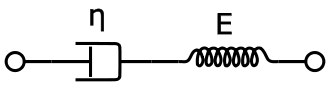
\includegraphics[width=0.5\textwidth]{figures/Maxwell-material.png}
    \caption{Schematische Darstellung des Maxwell - Materials}
    \label{fig:Maxwell-Material}
\end{figure}

Die resultierende Differentialgleichung fue;r die Schubspannung $\T$ nimmt folgende Form an:
%
\newnot{symbol:lambda}
\begin{equation}
    \label{eq:maxwellModell}
    \T + \lambda \frac{\partial\T}{\partial t}=2\eta \D
\end{equation}
Die Voraussetzung dafür ist dass das Stoffverhalten als linear angenommen wird, indem nur Verzerrungen mit hinreichend kleiner Amplitude betrachtet werden. Zusätzlich muss noch die Annahme eines exponentiell schwindenden Gedächtnisses getroffen werden, das heisst der Einfluss von Verzerrungen auf die aktuelle Spannung nimmt mit der Zeit exponentiell ab.
Wie schnell dieser Einfluss abnimmt, hängt dabei von der Relaxationszeit $\lambda$ ab.
%Wird dabei lineares Stoffverhalten vorausgesetzt indem nur Verzerrungen mit hinreichend kleiner Amplitude betrachtet werden, kann die Funktion $F$ in erster Näherung als linear betrachtet werden. Falls zusätzlich noch die Annahme eines schwindenden Gedächtnisses getroffen, das heisst der Einfluss von Verzerrungen auf die aktuelle Spannung nimmt mit der Zeit monoton ab, kann die Beziehung zwischen $\T$ und $\D$ als Integral

Eine Erweiterung dieses Modells ist das Oldroyd-B Modell, bei dem statt die partielle die kontravariante Ableitung $\overset{\nabla}{\T}$ verwendet wird:
\begin{equation}
    \label{eq:oldroydModell}
    \T + \lambda \overset{\nabla}{\T}=2\eta \D
\end{equation}
wobei
\begin{equation}
    \label{eq:upperconvectedDerivative}
    \overset{\nabla}{\T} = \frac{D}{Dt}\T-\left[ \nabla u^T\cdot \T \right]-\left[ \T\cdot \nabla u \right] 
\end{equation}
Diese Modifikation dient dazu, Drehungen und Verzerrungen des Fluides in der Differentialgleichung zu berue;cksichtigen.

Falls zusae;tzlich $\lambda$ und $\eta$ eine Funktion von $\gammap$ sein sollen, wird vom White-Metzner Modell gesprochen:
\begin{equation}
    \label{eq:whiteMetznerModell}
    \T + \lambda\left( \gammap \right) \overset{\nabla}{\T}=2\eta\left( \gammap \right) \D
\end{equation}
Dabei koe;nnen fue;r die Funktionen $\lambda$ und $\eta$ die selben Modelle wie fue;r die nicht Zeitabhae;ngigen Gesetze verwendet werden.
%
%\subsubsection{Strukturviskosität}
%%
%\subsubsection{Viskoelastizität}
%%
%\subsubsection{Konstitutive Gesetze}

\section{Numerische Verfahren}
\label{Kapitel:Numerik}
Für das Lösen der in Kapitel \ref{Kapitel:Rheologie} vorgestellten Gleichungen gibt es eine Vielzahl von Verfahren. In diesem Kapitel werden die in dieser Arbeit verwendeten Algorithmen vorgestellt.

\subsection{Semi-Implicit Method for Pressure-Linked Equations}
Der \textbf{S}emi-\textbf{I}mplicit \textbf{M}ethod for \textbf{P}ressure-\textbf{L}inked \textbf{E}quations (SIMPLE) Algorithmus \cite{cfd} ist eine Methode um das Druck- und Geschwindigkeitsfeld in einem inkompressiblen Fluid für eine stationäre Lösung zu berechnen.\\
Dabei wird abwechselnd eine Aktualisierung für den Druck und die Ge\-schwin\-dig\-keit berechnet. Über ein Konvergenzkriterium wird entschieden, wann die stationäre Lösung erreicht ist.\\
Ein Iterationsschritt des SIMPLE Algorithmus kann dabei wie folgt zusammengefasst werden:
\begin{outline}[enumerate]
    \1 Verwende eine Startlösung $p^*$
    \1 Ausgehend von $p^*$ berechne ein Geschwindigkeitsfeld $u^*$ mit Hilfe der (stationären) Impulsgleichung
    \1 Berechne eine Druckkorrektur $p^{'}$ durch das Lösen der Druckkorrekturgleichung $\nabla^2p=-\nabla \cdot \left( u^*\cdot\nabla \right)u^*$
    \1 Berechne ein neues Druckfeld $p^{**}=p^*+\alpha p^{'}$ wobei $\alpha \in (0,1]$ ein Unterrelaxationsparameter ist
    \1 Korrigiere die Geschwindigkeit um $\nabla u=0$ zu erfüllen.
\end{outline}

Der SIMPLE Algorithmus wurde in dieser Arbeit für die Simulation zeitunabhängiger nicht-Newtonscher Fluide benutzt. Dabei wurde der Ab\-hän\-gig\-keit der Viskosität $\eta$ von der Schergeschwindigkeit $\gammap$ Rechnung getragen, indem diese in jedem Iterationsschritt ausgewertet wurde. Dadurch ent\-steht im Vergleich zu der normalen Navier-Stokes Gleichung eine zu\-sätz\-liche nicht-Linearität. Dies beeinflusst das Konvergenzverhalten und muss bei der Wahl der Simulationsparameter wie z.B. Relaxationsfaktoren mit einbezogen werden.

\subsection{Pressure Implicit with Split Operator}
Der \textbf{P}ressure \textbf{I}mplicit with \textbf{S}plit \textbf{O}perator (PISO) \cite{cfd} Algorithmus ist ein Verfahren, um transiente Lösungen des Druck- und Geschwindigkeitsfeldes zu berechnen.\\
Ähnlich wie der \mbox{SIMPLE} Algorithmus wird dabei zwischen Druck und Ge\-schwin\-dig\-keit iteriert. Die Hauptunterschiede sind, dass keine Unterrelaxation angewendet wird, und dass die Impulsgleichung mehrfach gelöst wird:
%Ein Iterationsschritt beinhaltet also die selben Schritte wie im \mbox{SIMPLE} Algorithmus, mit folgenden Änderungen:
\begin{outline}[enumerate]
    \1 Verwende eine Startlösung $p^*$
    \1 Ausgehend von $p^*$ berechne ein Geschwindigkeitsfeld $u^*$ mit Hilfe der instationären Impulsgleichung
    \1 Berechne eine Druckkorrektur $p^{'}$ durch das Lösen der Druckkorrekturgleichung $\nabla^2p=-\nabla \cdot \left( u^*\cdot\nabla \right)u^*$
    \1 Berechne ein neues Druckfeld $p^{**}=p^*+ p^{'}$
    \1 Korrigiere die Geschwindigkeit um $\nabla u=0$ zu erfüllen.
    \1 Die Schritte 3-5 werden pro Zeitschritt eine vom Anwender bestimmte Anzahl mal ausgeführt
\end{outline}

\subsection{Discrete Elastic Viscous Split Stress}
Einer der Unterschiede zwischen zeitunabhängigen Fluiden und viskoelastischen Fluiden ist, dass der Spannungstensor nicht mehr nur eine Funktion des Geschwindigkeitsfeldes ist, sondern auch von der Zeit. Durch diese Zeitabhängigkeit muss er als unabhängige Variable betrachtet werden, für die auch Anfangs- und Randbedingungen vorgegeben werden müssen. Da\-durch wird das Lösen einer weiteren Gleichung notwendig.

Eine Möglichkeit für die stabile Diskretisierung dieser zusätzlichen Gleichung ist die \textbf{D}iscrete \textbf{E}lastic \textbf{V}iscous \textbf{S}plit \textbf{S}tress (DEVSS) Methode \cite{devss}.
Dabei wird die Hilfsvariable \nom[num:Ud]{$\underline{\D}$}{Hilfstensor des DEVSS Verfahrens} eingeführt, so dass 
\begin{equation}
    \label{eq:devss:d}
    \underline{\D} - \D= 0
\end{equation}
gilt. Nimmt man von \eqref{eq:devss:d} die Divergenz und subtrahiert das Resultat von der Impulsgleichung \eqref{eq:Impulserhaltung}, erhält man
\begin{equation}
    \label{eq:devss:impuls}
    \rho \u _t + \rho \u \cdot \nabla\u = -\nabla p +\nabla \cdot \T - a \nabla \cdot \left( \underline{\D}-\D \right).
\end{equation}
Hierbei ist \nom[num:a]{$a$}{Parameter des DEVSS Verfahrens} ein positiver Parameter.\\
Gleichung \eqref{eq:devss:impuls} kann umgeschrieben werden als
\begin{equation}
    \label{eq:devss:impuls2}
    \rho \u _t + \rho \u \cdot \nabla\u -a \nabla \cdot \D= -\nabla p +\nabla \cdot \T - a \nabla \cdot \left( \underline{\D} \right).
\end{equation}
Diese Null-Operation hat keinen Einfluss auf die Lösung des Gleichungssystems, ermöglicht aber durch eine unterschiedliche Diskretisierung von $\D$ und $\underline{\D}$ eine Stabilisierung des numerischen Problems.

Das iterative Verfahren zur Lösung der Gleichungen \eqref{eq:Massenerhaltung}, \eqref{eq:devss:impuls2} und \eqref{eq:Tviskoelastisch} lautet wie folgt:
\begin{outline}[enumerate]
    \1 Mit gegebenem Geschwindigkeitsfeld $u^*$, Druckfeld $p^*$ und Spannung $\tau^*$ wird die Impulsgleichung \eqref{eq:devss:impuls2} für ein neues Geschwindigkeitsfeld $u^{**}$ implizit gelöst
    \1 Durch Verwendung von $U^{**}$ wird eine neue Approximation des Druckfeldes $p^{**}$ berechnet und anschliessend eine Korrektur der Ge\-schwin\-dig\-keit mithilfe der Kontinuitätsgleichung durchgeführt um $u^{***}$ zu erhalten. Dazu wird der PISO Algorithmus verwendet.
    \1 $u^{***}$ wird benützt um mit Hilfe eines Konstitutiven Gesetzes \eqref{eq:Tviskoelastisch} ein neues Spannungsfeld $\tau^{**}$ zu erhalten.
    \1 Falls es sich um eine transiente Simulation handelt, können die Schritte 1-3 mehrmals pro Zeitschritt durchgeführt werden um eine genauere Lösung zu erhalten.
\end{outline}

\section{Simulationsframework}
\todo{Begriff Simulationsframework}
\label{Kapitel:Implementierung}
Die Implementierung der zugrunde liegenden Gleichungen und ihre Diskreti"-sierung wurde in \openfoam{} \cite{openfoam} realisiert.
\openfoam{} ist eine freie CFD Bibliothek für finite Volumen, in der zahlreiche Standardlöser schon implementiert sind und die es erlaubt auf eine einfache Art und Weise eigenen Code zu implementieren.\\
Für die Simulation der viskoelastischen Fluide wurde als Basis ein Code von J.~Favero \cite{faveroOF} verwendet, und an die in dieser Arbeit verwendeten Modelle und Gleichungen angepasst.

Die Notation in diesem Kapitel verwendet eine \fileemph{kursive Schrift} für Computer"-datei-Namen und eine \codeemph{Schreibmaschinenschrift} für Computercodes wie Programme oder Teile davon.

Ein Simulationslauf in \openfoam{} wird 'case' genannt, der durch ein Verzeichnis auf dem Computer repräsentiert wird. Da \openfoam{} keine gra\-phi\-sche Benutzeroberfläche besitzt, werden alle Informationen und Resultate in Textdateien gespeichert, die in diesem 'case' abgelegt werden.\\
Die Informationen sind aufgeteilt in die Unterverzeichnisse \fileemph{0}, \fileemph{constant} und \fileemph{system}, sowie Zeitschrittverzeichnisse die nach der jeweiligen Zeit benannt sind. Abbildung~\ref{fig:ofCaseSchema} zeigt die schematische Darstellung.\\ %In den darin gespeicherten Dateien stehen alle Informationen über die Simulation und deren Resultate.\\
Im Verzeichnis \fileemph{0} sind die Anfangs- und Randbedingungen der Simulation definiert. Die darin enthaltenen Dateien sind nach den entsprechenden Variablen genannt wie z.B. \fileemph{p} für den Druck oder \fileemph{U} für die Geschwindigkeit.
In \fileemph{constant} stehen die Simulationsparameter wie zum Beispiel das verwendete Viskositätsmodell und dessen Parameter. Ausserdem ist im Unterverzeichnis \fileemph{polymesh} die Geometrie definiert.
In \fileemph{system} sind schliesslich die Simulationskontrollgrössen enthalten. Dazu gehören in der Datei \fileemph{controlDict} die Anzahl der Zeitschritte und deren Länge, in \fileemph{fvSchemes} die verwendeten Diskretisierungsschemen und in \fileemph{fvSolution} welche Lösungsmethoden für die linearen Gleichungssystem verwendet werden.

\begin{figure}
    \centering
    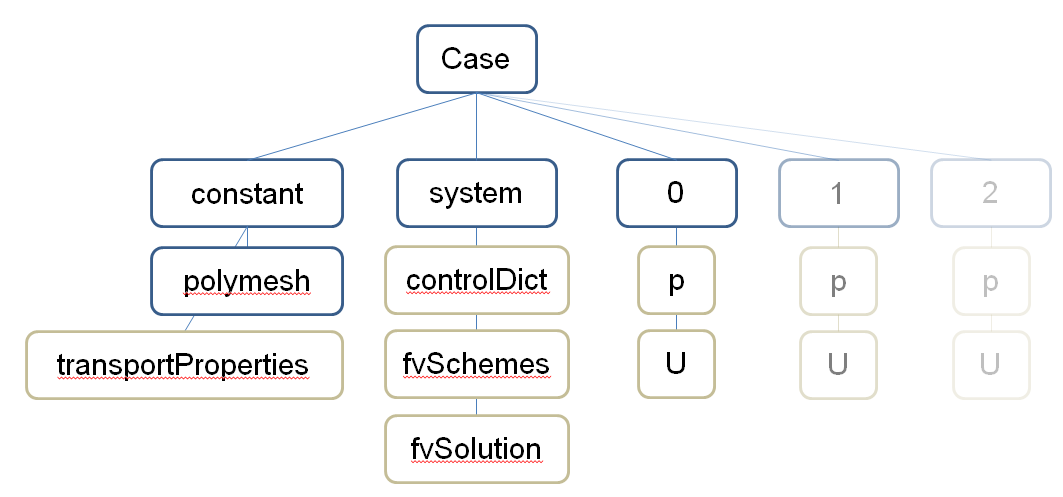
\includegraphics[width=\textwidth]{figures/OfCaseSchema.png}
    \caption{Der schematische Aufbau eines \openfoam{} 'cases'. Die blauen Einträge sind Verzeichnisse, die braunen stellen Dateien dar.}
    \label{fig:ofCaseSchema}
\end{figure}
%Die simulierten Mörtel weisen eine im Verhältnis zu den Strömungs"-geschwind"-ig"-keiten hohe Viskosität auf. 
%Die maximale Reynolds-Zahl die in in dieser Arbeit gemachten Simulationen auftritt ist im einstelligen Bereich, weshalb auf eine Turbulenz-Modellierung verzichtet und eine laminare Strömung vorausgesetzt wurde.
%
\subsection{Löser}
Ein Löser in \openfoam{} ist ein \cpp{} Programm, das in einem 'case' arbeitet. Der Löser ruft dabei die Informationen aus den im 'case' enthaltenen Verzeichnissen ab und benützt diese, um einen Simulationslauf zu definieren. Danach beginnt er die Simulation und erzeugt neue Zeitschritt-Verzeichnisse, in denen er den berechneten Zustand des Systems zu einem späteren Zeitpunkt abspeichert.

\subsubsection{simpleFoam}
Für die scherratenabhängigen Viskositätsmodelle wurde als Basislöser die schon in \openfoam{} eingebaute Version \codeemph{simpleFoam} des SIMPLE Algorithmus verwendet.
Diese erlaubt es unter verschiedenen schon implementierten Viskositätsmodellen zu wählen, oder diese zu modifizieren um ein eigenes Modell zu implementieren.\\
Dabei wird in der Datei \fileemph{transportProperties} als Transportmodell das gewünschte konstitutive Modell mit seinen Parametern hinterlegt:
%
\begin{lstlisting}
transportModel modifiedHerschelBulkley;

modifiedHerschelBulkleyCoeffs
{
    tau0        tau0  [ 0 2 -2 0 0 0 0 ] 343.0;
    k           k     [ 0 2 -1 0 0 0 0 ] 3.75;
    m           m     [ 0 0  1 0 0 0 0 ] 1000;
    n           n     [ 0 0  0 0 0 0 0 ] 0.848;
    nu0         nu0   [ 0 2 -1 0 0 0 0 ] 800;
}
\end{lstlisting}
%
\subsubsection{timeAdjustNonNewtIcoFoam}
Der Löser zu der in \openfoam{} implementierten Version des PISO Algorithmus heisst \codeemph{icoFoam}.
Diese Version unterstützt aber keine nicht-Newtonsche Modelle und ist nicht in der Lage, den Zeitschritt an die maximal auftretende Geschwindigkeit anzupassen.\\
Um trotzdem in der Lage zu sein nicht-Newtonsche, transiente Probleme zu lösen, wurde im Rahmen dieser Arbeit der Löser \codeemph{icoFoam} erweitert.

Analog zum Löser \codeemph{simpleFoam} wird zu Beginn der Simulation eine Instanz der Klasse \codeemph{transportModel} initialisiert, die dann in jedem Zeitschritt die kinematische Viskosität aktualisiert und zur Verfügung stellt:
%
\begin{lstlisting}
...
singlePhaseTransportModel fluid(U, phi);
...
while (runTime.run()) {
fluid.correct();
nu_ = fluid.nu();
}
...
\end{lstlisting}
%
Zusätzlich wurde in der Zeitschleife die von \openfoam{} zur Verfügung gestellte Routine \codeemph{setDeltaT.H} eingefügt, um $\Delta t$ in jedem Zeitschritt zu überprüfen und gegebenenfalls anzupassen.\\
Mit dieser Änderung können im \fileemph{controlDict} die Zeilen
%
\begin{lstlisting}
adjustTimeStep yes;
maxCo 0.5;
maxDeltaT 1;
\end{lstlisting}
%
eingefügt werden, um den Zeitschritt variabel zu machen.

Der resultierende Code \codeemph{timeAdjustNonNewtIcoFoam} ist in der Lage, sowohl mit nicht konstanten Viskositäten zu rechnen, als auch den Zeitschritt so zu wählen dass eine vom Nutzer bestimmte Courant Zahl nicht überschritten wird.\\
Die Courant oder auch CFL Zahl ist dabei definiert als Verhältnis zwischen Zeitschritt und räumlicher Auflösung und ist massgeblich für die Stabilität der Simulation
%
\begin{equation}
    c := \frac{\u\cdot \Delta t}{\Delta x} \overset{!}{<} 1.
\end{equation}
%
\subsubsection{viscoelasticFluidFoam}
Der Löser für die viskoelastischen Simulationen wurde von J.~Favero implementiert. Der Code ist eine Implementation des DEVSS Algorithmus, der aber für die Berechnung der Schubspannungsterme auf eine separat implementierte Klasse zurückgreift.\\
Dieser Code wurde unverändert übernommen und ist hier nur der Komplettheit halber aufgeführt.
%
\subsection{Rheologische Modelle}
Die rheologischen Modelle können in \openfoam{} als Bibliotheken eingebaut werden. Dazu wird ihr Code kompiliert und im \fileemph{controlDict} angegeben, welche Bibliotheken verwendet werden sollen. Sie sind keine eigenständigen Programme, sondern werden von den Lösern benutzt um Teile der Berechnung auszuführen.
%
\subsubsection{Scherratenabhängige Modelle}
Die Implementation eigener Modelle wurde realisiert indem eine neue \cpp{} Klasse implementiert wurde, die von der in \openfoam{} vorhandenen Klasse \codeemph{viscosityModel} abgeleitet ist.
Diese neue Klasse muss die Funktionen \codeemph{nu} und \codeemph{correct} zur Verfügung stellen. \codeemph{nu} gibt die die kinematische Viskosität zurück, \codeemph{correct} berechnet diese neu.
Dabei kann durch die von der Basisklasse zur Verfügung gestellte Funktion \codeemph{strainRate} auf die Scherrate $\gammap$ zurückgegriffen werden. Das Einlesen von zusätzlichen Parametern geschieht dabei in der Funktion \codeemph{read}.

Der schematische Aufbau solch einer Klasse:
%
\begin{lstlisting}
class limitedHerschelBulkley : public viscosityModel {
    tmp<volScalarField> nu() const {
        return nu_;
    }
    void correct() {
        nu_ = calcNu();
    }
    bool read(const dictionary& viscosityProperties) {
        ...
    }
};
\end{lstlisting}
%
In der Funktion \codeemph{correct} wird hier eine private Funktion \codeemph{calcNu} aufgerufen, die die Viskosität neu berechnet.
Das modifizierte Herschel-Bulkley Modell \eqref{eq:modHB} kann dabei, dank der sehr mächtigen Operatorüberladung von \openfoam{}, in einer sehr kompakten Schreibweise implementiert werden:
%
\begin{lstlisting}
Foam::tmp<Foam::volScalarField>
calcNu() {    
    return
    (
     min(
         nu0_,
         ( tau0_ * (1.001-exp(-1*m_*sr()))  + k_ *rtone* pow( tone*sr(),n_ ) )
         /(max(sr(), dimensionedScalar ("VSMALL", dimless/dimTime, VSMALL)))
        )
    );
}
\end{lstlisting}
%
wobei \codeemph{sr()} die Scherrate ist und \codeemph{tau0\_}, \codeemph{k\_} und \codeemph{n\_} die Modellparameter sind.\\
Durch die Division durch das Maximum der Scherrate und \codeemph{VSMALL}, einer sehr kleinen Konstante, wird die Division durch Null vermieden.\\
Da das Herschel-Bulkley Modell eine unendliche Viskosität vorsieht wenn das Fluide nicht geschert wird, dies aber zu numerischen Problem führen kann, wird ausserdem die Viskosität nach oben hin durch die Nullviskosität \codeemph{nu0\_} beschränkt.
%
\subsubsection{Viskoelastische Modelle}
Der Löser \codeemph{viscoelasticFluidFoam} greift für die Berechnung des Schubspannungtensors auf eine separate Klasse \codeemph{viscoelasticModel} zurück, die ähnlich der \codeemph{transportModel} Klasse in \codeemph{simpleFoam} die Methoden \codeemph{divTau} und \codeemph{correct} zur Verfügung stellt.\\
Die Methode \codeemph{divTau} berechnet dabei die Divergenz der Schubspannung $\T$ und implementiert gleichzeitig noch einen Teil der DEVSS Methodik indem sie die Split Stress Terme dazu addiert:
%
\begin{lstlisting}
Foam::tmp<Foam::fvVectorMatrix>
divTau(volVectorField& U) const {
    ...
    return
    (
        fvc::div(tau_/rho_, "div(tau)")
      - fvc::laplacian(etaPEff/rho_, U, "laplacian(etaPEff,U)")
      + fvm::laplacian( (etaPEff + etaS_)/rho_, U, "laplacian(etaPEff+etaS,U)")
    );
}
\end{lstlisting}

In der Methode \codeemph{correct} wird bestimmt, wie sich der Schubspannungstensor von einem Zeitschritt zum nächsten ändert.\\
Diese Methode ist der Teil der Klasse, der an das gewünschte viskoelastische Modell angepasst werden muss. Das in dieser Arbeit verwendete White-Metzner Modell \eqref{eq:whiteMetznerModell} benötigt für das Update des Schubspannungstensors drei Schritte.
In einem ersten Schritt müssen die direkt von $\u$ abhängigen Variablen berechnet werden
\begin{lstlisting}
volTensorField L = fvc::grad(U());
volTensorField C = tau_ & L;
volSymmTensorField twoD = twoSymm(L);
volScalarField gamma = sqrt(2.0) * mag(symm(L));
\end{lstlisting}

In einem zweiten Schritt werden die scherratenabhängige Relaxationszeit $\lambda$ und Viskosität $\eta$ aktualisiert
\begin{lstlisting}
volScalarField etaPValue =
     max(
         etaMin_,
         min(
             etaMax_,
             ( tau0_ + K_ * rtone * Foam::pow( tone*gamma,n_ ) )
             /(max(gamma, dimensionedScalar ("VSMALL", dimless/dimTime, VSMALL)))
         )
     );

volScalarField lambdaValue = 
        lambdaInf_+(lambdaNull_-lambdaInf_) * 
                Foam::pow(
                1 + Foam::pow( L_* gamma,b_), 
                (nLambda_- 1)/b_
                );
\end{lstlisting}
%
Als letztes wird die Differentialgleichung mit dem Transport-Term implizit gelöst
%
\begin{lstlisting}
fvSymmTensorMatrix tauEqn
(
    fvm::ddt(tau_)
    + fvm::div(phi(), tau_)
    ==
    etaPValue/lambdaValue*twoD
    + twoSymm(C)
    - fvm::Sp(1/lambdaValue, tau_)
);
           
tauEqn.relax();
tauEqn.solve();
\end{lstlisting}
%
\subsection{Post processing}
Für die Auswertung der Simulationen gibt es mit ParaView \cite{paraview} und diversen \openfoam{} Utilities schon eine ganze Anzahl von Möglichkeiten.\\
In dieser Arbeit wurde zusätzlich noch die Möglichkeit genutzt eigene Runtime Functions zu schreiben, also Funktionen die schon während der Simulation bestimme Werte berechnen und damit Einblick in die laufende Simulation ermöglichen.
%
\subsubsection{patchAverage}
Die Funktion \codeemph{patchAverage} ist eine vereinfachte Version der schon in \openfoam{} implementierten Runtime Function \codeemph{fieldValue}.\\
Sie dient dazu, in vom Nutzer bestimmten Zeitabständen ein bestimmtes Feld über eine oder mehrere Randflächen der simulierten Geometrie zu mitteln und das Resultat in eine separate Datei zu speichern.\\
Ein Beispiel für die Anwendung ist das Beobachten des mittleren Einlassdruckes bei festgelegter Einlassgeschwindigkeit in einer Strömung.\\
Dazu müssen im \fileemph{controlDict} folgende Zeilen hinzugefügt werden:
%
\begin{lstlisting}
functions
(
    DruckAmEinlass {
        type averageValue ;
        functionObjectLibs (``libaverageValue.so'');
        patches (Einlass);
        outputControl timeStep;
        fields (p)
    }
);
\end{lstlisting}
%
Dadurch wird in jedem Zeitschritt die Funktion \codeemph{calcAverageValues} aufgerufen, die über alle Felder und Flächen iteriert und den Durchschnitt berechnet:
%
\begin{lstlisting}
forAll(fieldNames_, fieldi) {    
forAllConstIter(labelHashSet,patchSet_, iter) {
    label patchi = iter.key();
    // add this patch's area to the sum
    areas[fieldi] += sum(mesh.magSf().boundaryField()[patchi]);
    // multiply face area with face-value and sum up.
    avgVals[fieldi] +=
        sum(mesh.magSf().boundaryField()[patchi]*f.boundaryField()[patchi]);
    avgVals[fieldi] /= areas[fieldi];
}
return avgVals;
}
\end{lstlisting}
%
\subsubsection{torqueCalc}
Im Kapitel \ref{Kapitel:Korrektursimulation} wird beschrieben, wie die Viskosität des Mörtels anhand des Drehmomentes in einem Platte-Platte Rheometer bestimmt wird.\\
Die Berechnung dieses Drehmomentes kann zwar mit den schon vorhandenen Utilities in \openfoam{} durchgeführt werden, allerdings ist das eher umständlich und es müssen mehrere Funktionen aufgerufen werden.\\
Um das zu vermeiden, wurde die Funktion \codeemph{torqueCalc} geschrieben, die das Drehmoment in jedem Zeitschritt berechnet.
Dadurch ist nicht nur die Auswertung der Simulation einfacher, es kann durch eine Überprüfung der Änderung des Drehmoments auch eine Konvergenzbedingung angegeben und die Simulation in jedem Zeitschritt beendet werden.

Die Implementierung wurde ebenfalls als runtime function umgesetzt. In der Funktion \codeemph{calcTorque} wird das Drehmoment $M$ an den vom Nutzer bestimmten Randflächen $A_i$ berechnet:
\newnot{symbol:M}
\begin{equation}
    M = \sum_i \int_{A_i}r\tau\left( r \right)dA_i
\end{equation}
wobei 
\begin{equation}
    \tau\left( r \right) = \nu\left( r \right) \cdot \frac{\partial \u\left( r \right)}{\partial \n\left( r \right)}
\end{equation}
die Schubspannung an der Wand und $r$ der Abstand zum Rotationszentrum ist.

In \openfoam{} kann die Schubspannung mithilfe der schon implementierten Funktion \codeemph{snGrad} sehr einfach berechnet werden, wobei die Viskosität erst später dazu multipliziert wird:
%
\begin{lstlisting}
wallShearStress = vel.boundaryField()[patchi].snGrad();
\end{lstlisting}

Der Abstand $r$ ist die X-Komponente eines lokalen Zylinder-Koordinatensystems
\begin{lstlisting}
cylindricalCS ccs
(
 "ccs",
 vector(0,0,0), // Origin
 vector(0,1,0), // Cylindrical axis
 vector(1,0,0)  // Vector with zero angle
);
\end{lstlisting}

Die Summe und das Integral über die vorgegebenen Flächen kann dann mittels einer for-Schleife implementiert werden:
\begin{lstlisting}
forAllConstIter(labelHashSet,patchSet_, iter)
{
 label patchi = iter.key();
 torque+= sum
 (
  ccs.localVector(wallShearStress)().
       component(vector::X) *
  transportModel.nu()().
       boundaryField()[patchi] * 
  ccs.localVector(mesh.C().boundaryField()[patchi])().
       component(vector::X) *
  mesh.magSf().boundaryField()[patchi]
 );
}
\end{lstlisting}

Die Konvergenzbedingung ist in der Funktion \codeemph{checkConvergence} eingebaut.
Dabei wird für das Berechnen der ersten und der zweiten Ableitung die finite Differenzen Methode benutzt:
%
\begin{eqnarray}
    \label{eq:torqueCalc:fd}
    \dot{m} & = & \frac{1}{2}\left(  m[t+1] - m[t-1] \right) \\
    \ddot{m} & = & \frac{1}{2}\left(  m[t+1] - 2 \cdot m[t] + m[t-1] \right) 
\end{eqnarray}
%
Die Werte $m[t]$ wurden dabei in einer \codeemph{fixedList} der Grösse drei gespeichert, in die jeweils periodisch die neuen Werte geschrieben werden
%
\begin{lstlisting}
label ip1 = convListIt_;
label i   = convList_.rcIndex(ip1);
label im1 = convList_.rcIndex(i);
scalar firstDeriv = (convList_[ip1]-convList_[im1])/2;
scalar secondDeriv = (convList_[ip1]-2*convList_[i]+convList_[im1]);

if (mag(firstDeriv) < convergence_ && mag(secondDeriv) < convergence_/100)
{
    Info << "Convergence reached, stopping simulation now" << nl;
    obr_.time().stopAt(Time::saWriteNow);
}
\end{lstlisting}
%
%
%\begin{lstlisting}
%scalar torque = calcTorque();

%convList_[convListIt_]=torqü
%// Get next index (periodic)
%convListIt_=convList_.fcIndex(convListIt_);
%\end{lstlisting}
%
\subsection{Betriebssystem und Hardware}
\label{Kapitel:Hardware}
\openfoam{} kann nicht unter Windows verwendet werden, da es eine Unterscheidung zwischen Gross- und Kleinschreibung bei Dateinamen benötigt. Die in dieser Arbeit verwendeten Betriebssysteme sind deshalb Linux-Distributionen.

Für kleinere lokale Berechnungen und Testläufe stand ein Laptop zur Verfügung, auf dem Ubuntu 12.04 LTS installiert wurde.
Der Hauptteil der Simulationen wurde aber auf den HPC-Clustern des Swiss National Supercomputing Centre (CSCS) durchgeführt.
Mit dem im Tessin gelegenen Cluster Rothorn stand ein Berechnungsknoten mit 256 CPUs zur Verfügung. Das System ist ein SGI Altix UV 1000, das für Berechnungen einen Arbeitsspeicher von 2TB besitzt.
Das Betriebssystem ist SUSE SLES11 SP1, wobei die Bedienung über eine 'secure shell' (ssh) Verbindung geschieht.

Die visuelle Nachbearbeitung der Resultate wurde ebenfalls beim CSCS gemacht, allerdings nicht auf Rothorn sondern auf einem Dalco SM System, das Eiger genannt wird.\\
Da die Visualisierung eine graphische Benutzeroberfläche benötigt, geschieht die Bedienung nicht über ssh, sondern durch eine 'virtual network computing'-Verbindung, die die Bildschirmausgabe des entfernten Computers auf eine lokale Maschine überträgt und im Gegenzug Maus- und Tastatureingaben zurück sendet.

\section{Model Parameter}
\label{Kapitel:Parameter}
Um eine moe;glichst realistische Simulation zu ermoe;glichen, ist es notwendig die verwendeten Modelle moe;glichst genau an Messdaten der realen Moe;rtel anzupassen.
Für einige der Mörtel wurden die Parameter, die im verwendeten Modell \eqref{eq:modHB} vorkommen, schon bestimmt. \\
Einerseits wurden aber in der Zwischenzeit neue Mörtel entwickelt und andererseits ist es wünschenswert, ein Tool zur Bestimmung dieser Parameter zu haben das unabhängig von Drittanbietern in Form von Lizenzen und Support ist. \\
Dies wurde mithilfe einer Kombination aus \openfoam{} und der Programmiersprache Python umgesetzt.
%
\subsection{Messaufbau}
Die Messungen wurden von einem Hilti-internen Rheologen durchgefue;hrt. Verwendet wurden zwei Messgerae;te, ein Platte-Platte Rheometer und ein Kapillarrheometer.
%
\subsubsection{Platte-Platte Rheometer}
\label{Kapitel:Parameter:PlattePlatteRheo}
Ein Platte-Platte Rheometer ist ein Messgerae;t zur Bestimmung der Viskositae;t eines Fluids abhae;ngig von der Scherrate.\\
Die Flue;ssigkeit wird zwischen zwei Platten platziert, von denen die eine Fix ist und die andere mit einer vorgegebenen Geschwindigkeit gedreht wird.
Dabei wird das benoe;tigte Drehmoment gemessen, das fue;r die Drehgeschwindigkeit aufgewendet werden muss.
\todo{Formeln Berechnung Viskositaet}

Das Platte-Platte Rheometer eignet sich ebenfalls dazu, zeitabhae;gige Effekte wie die Relaxationszeit eines viskoelastischen Fluids zu messen. 
Dazu wird die obere Platte nicht mit einer konstanten Geschwindigkeit bewegt, sondern mit einer schwingungsae;hnlichen Drehung auf die eine oder die andere Seite gedreht.
%
\begin{todocontent}
    \1 Beschreibung Rheometer
    \1 Bilder von Messkurven
\end{todocontent}
%
\subsubsection{Kapillarrheometer}
Das Kapillarrheometer kann wie das Platte-Platte Rheometer zur Bestimmung der scherratenabhae;ngigen Viskositae;t verwendet werden. Das Fluid wird dabei aber nicht gedreht, sondern durch eine schmale Due;se gepresst
\todo{Formeln Kapillarrheometer}
\begin{todocontent}
    \1 Beschreibung Rheometer
    \1 Bilder von Messkurven
\end{todocontent}
%
\subsection{Korrektursimulation}
\label{Kapitel:Korrektursimulation}
Die in Kapitel \ref{Kapitel:Parameter:PlattePlatteRheo} beschriebenen Rheometer messen das fue;r eine vorgegebene Geschwindigkeit benoe;tigte Drehmoment. Daraus kann die Viskositae;t des Fluides berechnet werden.\\
Um zu verhindern, dass der Moe;rtel wae;hrend der Messung in radialer Richtung davon fliesst, wurde um das Rheometer herum ein Ring montiert. Dadurch wird zwar ein Herausfliessen verhindert, gleichzeitig wird aber die Messung verfae;lscht. Der Ring ist eine zusae;tzliche Wand an der das Fluid entlangstroe;men muss, was in einem erhoe;hten Drehmoment resultiert.

Um trotzdem eine zuverlae;ssige Bestimmung der Modell-Parameter zu ermoe;glichen, ist es notwendig diesen Ring im Fit zu berue;cksichtigen. Dazu wird nicht die gemessene Viskositae;t verwendet, sondern versucht die Modell-Parameter so zu wae;hlen dass eine Simulation des Platte-Platte Rheometers eine moe;glichst genaue Approximation des Drehmoments ergibt.

Beim Platte-Platte Rheometer handelt es sich um eine rotationssymmetrische Geometrie. Um Rechenzeit zu sparen wurde deshalb nur ein schmaler Ausschnitt der Geometrie simuliert, wie im Bild (x) \todo{figure Netz Platte Rheo} zu sehen ist.\\
%
\subsection{Parameterfit}
Die in Kapitel \ref{Kapitel:Korrektursimulation} beschriebene Wahl der Parameter ist ein nichtlineares Ausgleichsproblem. Dabei soll die Gleichung \eqref{eq:modHB} moe;glichst gut an Mess- und Simulationsdaten gefittet werden, indem die Parameter $\tau_0$, $K$ und $n$ variiert werden.

Fue;r die Loe;sung dieses Ausgleichproblemes wurde die Programmiersprache Python verwendet. Die Tatsache dass sie, ebenso wie \openfoam{}, frei verfue;gbar \todo{Lizenz abklaeren} ist und dass es unzae;hlige schon implementierte numerische Algorithmen gibt machen Python zur idealen Wahl dafue;r.

Die Optimierung wurde als Python Modul \codeemph{MaT\_Optimizer} implementiert. Dabei wurde auf die Bibliotheken \codeemph{Numpy} und \codeemph{Scipy} \todo{referenz} zurue;ckgegriffen um verschiedene Standardfunktionen zur Verfue;gung zu haben.\\
Das Ausgleichsproblem wird dabei mittels der Funktion \codeemph{leastsq} aus dem Modul \codeemph{optimize} von \codeemph{Scipy} geloe;st. Diese Funktion ist eine Implementierung des Levenberg-Marquardt Algorithmus, der das Problem auf eine iterative Weise loe;st.

Dazu wird eine eine enge Kopplung von Python und \openfoam{} noe;tig, da die Auswertung der Funktion, an die gefittet werden soll, eine Reihe von Simulationen ist.
Diese Kopplung wurde dabei mit Hilfe von \codeemph{PyFoam} \todo{Referenz} realisiert. \codeemph{PyFoam} ist eine Python Bibliothek die es ermoe;glicht, die von \openfoam{} als Ein- und Ausgabe benutzten Textdateien auf eine einfache Art und Weise zu erzeugen, zu ae;ndern und auszulesen.

Um den Prozess der Parameter-Optimierung zu beschleunigen, wurde ausserdem die Bibliothek \codeemph{Parallel Python} \todo{Referenz} verwendet. Da eine Funktionsauswertung aus einer ganzen Reihe Simulationen besteht, wird dazu viel Zeit benoe;tigt. Diese Simulationen sind aber unabhae;ngig voneinander und koe;nnen deshalb sehr einfach parallelisiert werden. Mit \codeemph{Parallel Python} koe;nnen beliebig viele Prozessoren fue;r den Parameterfit verwendet werden.
%
\begin{todocontent}
    \1 Verwendung Python
    \1 Kopplung Python <-> OpenFOAM
    \1 Parallelisierung
    \1 Kapillarrheometerdaten
    \1 Vergleich mit alten Daten
\end{todocontent}
%
\subsection{Ergebnisse}
\begin{todocontent}
    \1 Kapillarrheometer Netze
    \1 Vergleich Platten und Kapillarrheometer unter Verwendung der errechneten Daten
    \1 Einfluss Netze
    \1 Einfluss Viskoelastiziaet
\end{todocontent}
%

\section{Hilti Auspressgerät}
\label{Kapitel:Auspressgeraet}
Die von Hilti hergestellten chemischen Due;bel werden mit einem eigens dafue;r entwickelten Auspressgerae;t in gebohrte Loe;cher gedrue;ckt. Dieses Auspressgerae;t soll gleichzeitig moe;glichst zuverlae;ssig und stabil sein, aber auch so konstruiert dass fue;r die Anwendung wenig Kraft gebraucht wird und exakt so viel Fluid ausgepresst wird wie vom Anwender gewollt.\\
Das derzeit auf dem Markt erhae;ltliche Gerae;t ist in Abbildung \ref{fig:Auspressgeraet} gezeigt.
%
\begin{figure}
    \centering
    \subfigure[Handgerae;t]{
        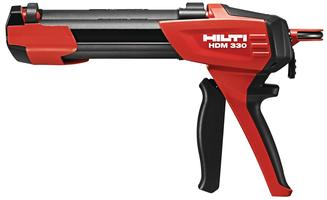
\includegraphics[width=0.31\textwidth]{figures/Auspressgeraet.jpg}
        \label{fig:Auspressgeraet:subA}
    }
    \subfigure[Akkugerae;t]{
        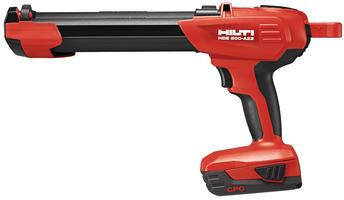
\includegraphics[width=0.31\textwidth]{figures/AuspressgeraetAkku.jpg}
        \label{fig:Auspressgeraet:subB}
    } 
    \subfigure[Moe;rtel Kartusche]{
        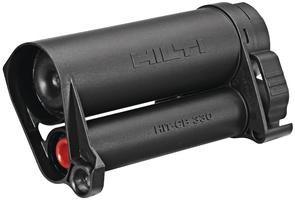
\includegraphics[width=0.31\textwidth]{figures/AuspressgeraetKasette.jpg}
        \label{fig:Auspressgeraet:subC}
    }
    \caption{Das Gerae;t zum Auspressen von Hilti Injektionsmoe;rtel. In \subref{fig:Auspressgeraet:subA} ist das Handgerae;t zu sehen, in \subref{fig:Auspressgeraet:subB} die Ausfue;hrung mit Akku, bei der das Auspressen auf Knopfdruck geschieht.\\
    In \subref{fig:Auspressgeraet:subC} ist eine Kartusche abgebildet, in die die Moe;rtelbeutel gelegt werden.}
    \label{fig:Auspressgeraet}
\end{figure}
%

Da die verwendeten Moe;rtel jeweils aus zwei Komponenten bestehen, mue;ssen sie bei der Anwendung gemischt werden. Dies geschieht in einem Mischer, der vorne am Auspressgerae;t angeschraubt wird. (Abbildung \ref{fig:Mischer})\\
%
\begin{figure}
    \centering
    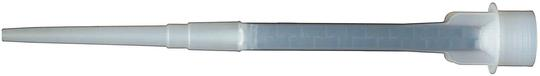
\includegraphics[width=0.8\textwidth]{figures/Mischer.jpg}
    \caption{Das Mischermodell HIT-RE-M, in dem die Moe;rtel nach dem Auspressen gemischt werden.}
    \label{fig:Mischer}
\end{figure}
%
Dieser Mischer kann jeweils nur einmal verwendet werden, weil der Moe;rtel ab dem Zeitpunkt des Mischens beginnt sich zu erhae;rten und so beginnt den Mischer zu verstopfen sobald das Auspressen gestoppt wird. Es ist deshalb im Interesse des Verbrauchers, dass der Mischer im Erwerb sehr preiswert ist. Trotzdem soll er natue;rlich die Komponenten moe;glichst gut mischen, da dies entscheidend fue;r die maximale Zuglast der Due;bel ist.

Diese Ansprue;che an das Gerae;t und den Mischer erfordern ein hohes Mass an Verstae;ndnis fue;r die Vorgae;nge wae;hrend dem Auspressen, weshalb sie in der Forschungsabteilung von Hilti stae;ndig weiter vermessen, simuliert und verbessert werden.
%
\subsection{Messaufbau}
Das fue;r die Moe;rtel verwendete Auspressgerae;t besteht zum groe;ssten Teil aus Kunststoff. Da dieser selber elastische Eigenschaften besitzt, ist es sehr schwierig die viskoelastischen Eigenschaften eines Fluides zu bestimmen, das durch das Geraet fliesst.\\
Um einen Einfluss des Gerae;tes auf das Fluid auszuschliessen, wurde deshalb die Geometrie des Auspressgerae;tes in einer sogenannten Funktionsersatzprue;fung (FEP) aus Metall nachgebaut. In Abbildung \ref{fig:FEP} sind Bilder dieser FEP zu sehen.
%
\begin{figure}
    \centering
    \subfigure[Metallnachbau]{
        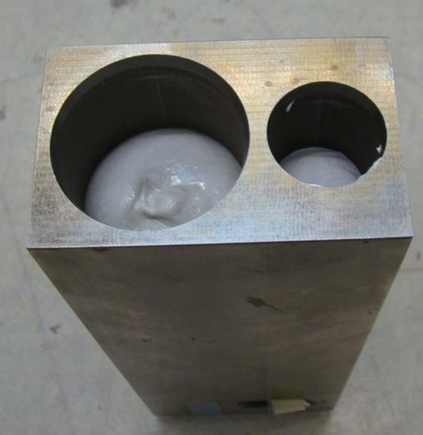
\includegraphics[width=0.31\textwidth]{figures/FEP_1.png}
        \label{fig:FEP:subA}
    }
    \subfigure[mit Moe;rtel gefue;llt]{
        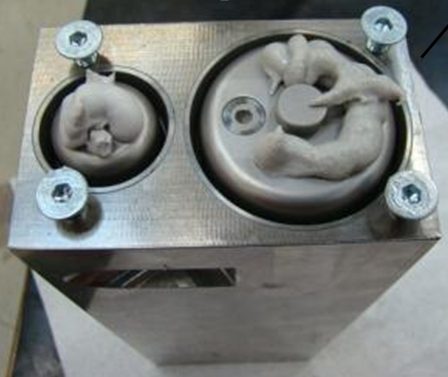
\includegraphics[width=0.31\textwidth]{figures/FEP_2.png}
        \label{fig:FEP:subB}
    } 
    \subfigure[Übergang zwischen Kolben und Mischer]{
        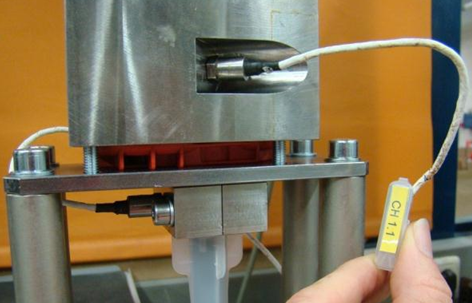
\includegraphics[width=0.31\textwidth]{figures/FEP_3.png}
        \label{fig:FEP:subC}
    }
    \caption{Der Messaufbau fue;r das Auspressgerae;t. In Abbildung \subref{fig:FEP:subA} ist der Nachbau der Geometrie aus Metall zu sehen, der in \subref{fig:FEP:subB} mit Moe;rtel befue;llt worden ist.\\
    Dieser Moe;rtel wird dann von einem Kolben durch eine Blende in den Mischer gepresst, der Übergang ist in \subref{fig:FEP:subC} zu sehen.}
    \label{fig:FEP}
\end{figure}
%
\subsection{Simulation}
\begin{todocontent}
    \1 Verwendete Netze
    \1 Loeserparameter (Relaxation)
    \1 Anfangsloesung wichtig fuer Konvergenz
\end{todocontent}
%
\subsection{Resultate}
\begin{todocontent}
    \1 Resultat Simulation (Bilder)
    \1 Druckvergleich
    \1 Einfluss Viskoelastizitaet
\end{todocontent}

\section{Zusammenfassung und Ausblick}
\label{Kapitel:Outlook}
In dieser Arbeit wurden zwei von der Firma Hilti AG in der Befestigungstechnik verwendete Mörtel mittels numerischer Simulationen untersucht.
Ziel der Arbeit war, die Fliess"-vorgänge dieser rheologisch komplexen Mörtel mithilfe der Simulationssoftware \openfoam{} zu modellieren. Dies soll das für die Produktentwicklung entscheidende Verständnis dieser Fliess"-vorgänge verbessern.

Die untersuchten Mörtel zeigen dabei ein starkes nicht-Newtonsches Verhalten.
Dies äussert sich sowohl in einer Scherverdünnung (Struktur"-viskosität), als auch in viskoelastischen Phänomenen. Die Modellierung dieser Eigenschaften geschah mit den empirischen Modellen Herschel-Bulkley, Carreau-Yasuda und White-Metzner.\\
Die grundlegenden Gleichungen, bestehend aus den Erhaltungssätzen für Masse und Impuls und den aus den Modellen resultierenden Schliessungsansätzen, wurden numerisch gelöst. Die benötigten numerischen Verfahren und Routinen wurden als Computercodes in \openfoam{} implementiert.

Die für die Modelle notwendigen Materialparameter wurden mithilfe eines in Python implementierten Optimierungsverfahren an Messdaten angepasst. Diese Daten stammen von zwei verschiedenen Rheometern, einem Platte-Platte Rheometer und einem Kapillarrheometer.
Die Verfälschung der Platte-Platte Rheometerdaten durch einen um den Scherspalt herum montierten Ring wurde durch eine entsprechende Korrektursimulation ausgeglichen.
Die Verifizierung der verwendeten Modelle und der berechneten Parameter geschah mittels Simulationen des Kapillarrheometers, bei denen eine gute Übereinstimmung mit der Realität gefunden wurde.

\begin{todocontent}
    \1 Einfluss Viskoelastizität
\end{todocontent}

Die Validierung geschah anhand eines anwendungsnahen Strömungsversuches. Dabei wurde eine vereinfachte Nachbildung des realen Auspressgerätes für die Hilti Mörtel gebaut und vermessen, um Einflüsse die ihren Ursprung nicht in Eigenschaften des Fluids haben auszuschliessen.
Die Geometrie dieser Funktionsersatzprüfung wurde im Computer nachgebildet und für die Strömungssimulation benützt.

Die Resultate zeigen tendenziell ein richtiges Verhalten, eine genaue Nachbildung der Druckverluste in der Funktionsersatzprüfung schlug aber fehl. Die Gründe für die Abweichungen konnten im Rahmen dieser Arbeit aus Zeitgründen nicht abschliessend erklärt werden. Denkbar ist, dass der Mörtel eine in der Simulation nicht berücksichtigte Temperaturabhängigkeit besitzt, oder dass verschiedene Produktions-Chargen unterschiedliche Fliesseigenschaften haben. Auch eine eventuelle Thixotropie der Mörtel wurde nicht in die Berechnung mit einbezogen.

Eine mögliche Erweiterung dieser Arbeit ist deshalb der Einbau von thixotropen Effekten.
Die verwendeten Algorithmen für die viskoelastischen Berechnungen benötigen noch eine grosse Anzahl an Iterationsschritten um zu konvergieren, weshalb hier ebenfalls noch Verbesserungs"-bedarf besteht.

Der Firma Hilti steht mit den programmierten Routinen ein Grundgerüst zur Verfügung, mit dem sie in Zukunft weitere Materialmodelle und -parameter verwenden kann um die Fliessvorgänge in ihrem Auspressgerät noch besser zu verstehen.

%\section{Section}
\label{section}

\subsection{Subsection}
\label{subsection}

\subsubsection{Notation, Todo and Citation}
\label{notation}
There is a stopping region $\Gamma_S$ \newnot{symbol:GammaS} of width $\delta>0$. \newnot{symbol:delta}
\cite{boehme}
\todo{add a picture here}

\subsubsection{Code}
Code:
\begin{lstlisting}
void Scheduler<SchedulingAlgorithm, spacedimV>::schedule(){
// Get number of available cores
int nCores = MPI::COMM_WORLD.Get_size();

// Create instance of scheduling algorithm
SchedulingAlgorithm schedulAlgo;
// And call its scheduling method
schedulAlgo.schedule( 
        // number of available cores
        nCores,
        // List with problem weights, problem i has a computational complexity of problemSizes[i]
        problemSizes,
        // List of lists to be filled with the scheduling, problem i is calculated on all cores contained in the list problemToCore[i]
        problemToCore
);

}
\end{lstlisting}

\subsubsection{Outline}
Example of outline:
\begin{outline}
    \1 First level
        \2 Second level
            \3 Third level
        \2[+] Second level with custom symbol
    \1 Again first level
        \2[] Second level without symbol
\end{outline}
\begin{outline}[enumerate]
    \1 Numerated outline
        \2 Second level
            \3 Third level
\end{outline}

\subsubsection{Pictures}
Example of subfloats with separate labeling:
Figure~\ref{fig:strongscalingfull} shows the timing \subref{fig:sub:strongscalingfulltiming} and the efficiency plot \ref{fig:sub:strongscalingfullefficiency} for the RTE solver with the full tensor solution method.
\begin{figure}[h]
    \centering
    \subfloat[Timings]{
        \includegraphics[height=40mm]{figures/strongscalingfulltiming.png}
        \label{fig:sub:strongscalingfulltiming}
    }
    \subfloat[Efficiency]{
        \includegraphics[height=40mm]{figures/strongscalingfullefficiency.png}
        \label{fig:sub:strongscalingfullefficiency}
    }
    \caption{Strong scaling of the RTE solver with the full tensor method. On the left the timing results are shown, on the right the according efficiency numbers are plotted.}
    \label{fig:strongscalingfull}
\end{figure}

\subsubsection{todocontent}
The todocontent environment is a customizable outline environment to help making the outline of a text.
\begin{todocontent}
    \1 This chapter should contain information about cows
    \1 And not to forget milk!
\end{todocontent}


\backmatter
%%% Bibliography
%\bibliographystyle{ThesisStyleWithEtAl}
%\bibliographystyle{ThesisStyle}
\bibliographystyle{plain}
\bibliography{sources}

\end{document}
